% diagrams/english/calabaza.tex -- la calabaza de Halloween, para "Read
% and colour": la calabaza (tres gajos: los dos de los lados asoman
% detrás del de en medio), el tallo, y los ojos y la sonrisa recortados
% en el gajo de en medio, por donde sale la luz de dentro.
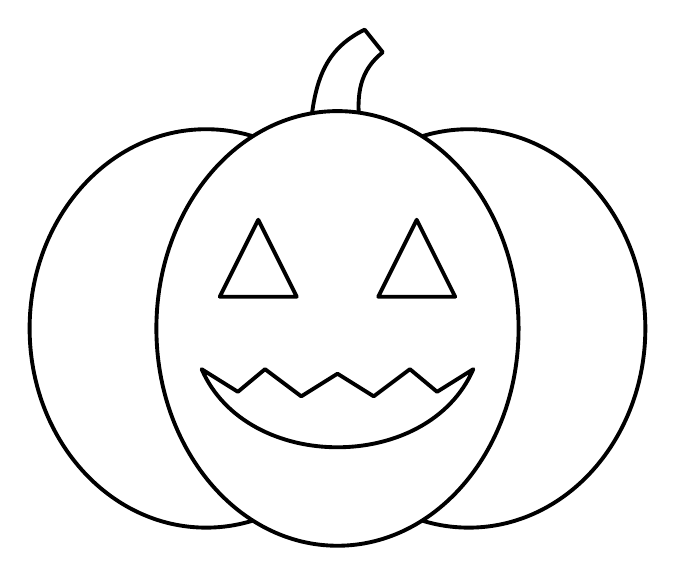
\begin{tikzpicture}[line width=1.4pt, line cap=round, line join=round, scale=1.15]
  % el tallo
  \filldraw[fill=white] (-0.3,2.2) .. controls (-0.25,2.8) and (-0.1,3.1) .. (0.3,3.3)
    -- (0.5,3.05) .. controls (0.25,2.85) and (0.2,2.6) .. (0.25,2.2) -- cycle;
  % los gajos de los lados y el de en medio
  \filldraw[fill=white] (-1.45,0) ellipse (1.95 and 2.2);
  \filldraw[fill=white] (1.45,0) ellipse (1.95 and 2.2);
  \filldraw[fill=white] (0,0) ellipse (2.0 and 2.4);
  % los ojos, dos triángulos
  \filldraw[fill=white] (-1.3,0.35) -- (-0.45,0.35) -- (-0.875,1.2) -- cycle;
  \filldraw[fill=white] (0.45,0.35) -- (1.3,0.35) -- (0.875,1.2) -- cycle;
  % la sonrisa
  \filldraw[fill=white] (-1.5,-0.45) -- (-1.1,-0.7) -- (-0.8,-0.45) -- (-0.4,-0.75)
    -- (0,-0.5) -- (0.4,-0.75) -- (0.8,-0.45) -- (1.1,-0.7)
    -- (1.5,-0.45) .. controls (1.0,-1.6) and (-1.0,-1.6) .. (-1.5,-0.45) -- cycle;
\end{tikzpicture}
